\documentclass{article}
\usepackage[cm]{fullpage} %very small margins (around 1.5cm)
\usepackage[utf8]{inputenc} %sets input encoding to UTF-8, needed for Polish, Japanese, etc.
\usepackage[T1]{fontenc} %needed for Polish characters
\usepackage{lmodern} %this font handles Polish characters properly

\PassOptionsToPackage{usenames,dvipsnames,svgnames}{xcolor}

%this file must be included in the preamble

\usepackage{graphicx} %use \includegraphics[scale=1.00]{file.jpg} for images
\usepackage[unicode]{hyperref}

\hypersetup{
  bookmarksopen,
  bookmarksopenlevel=1,
  pdfborder={0 0 0},
  %pdfpagelayout={SinglePage},
  %pdfstartview={FitH},
  pdfdisplaydoctitle
}

\def\logoleft#1{\gdef\logoleftpath{#1}}
\def\logoleftpath{\errmessage{Please define the logoleft}}

\def\logoleftscale#1{\gdef\logoleftscaletext{#1}}
\def\logoleftscaletext{\errmessage{Please define the logoleftscale}}

\def\logoright#1{\gdef\logorightpath{#1}}
\def\logorightpath{\errmessage{Please define the logoright}}

\def\logorightscale#1{\gdef\logorightscaletext{#1}}
\def\logorightscaletext{\errmessage{Please define the logorightscale}}

\def\title#1{\gdef\titletext{#1}\hypersetup{pdftitle={#1}}}
\def\titletext{\errmessage{Please define the title}}

\def\author#1{\gdef\authortext{#1}\hypersetup{pdfauthor={#1}}}
\def\authortext{\errmessage{Please define the author}}

\def\supervisor#1{\gdef\supervisortext{#1}}
\def\supervisortext{\errmessage{Please define the supervisor}}

\def\date#1{\gdef\datetext{#1}}
\def\datetext{\errmessage{Please define the date}}

\def\university#1{\gdef\universitytext{#1}}
\def\universitytext{\errmessage{Please define the university}}

\def\faculty#1{\gdef\facultytext{#1}}
\def\facultytext{\errmessage{Please define the faculty}}

\def\location#1{\gdef\locationtext{#1}}
\def\locationtext{\errmessage{Please define the location}}

\def\description#1{\gdef\descriptiontext{#1}}
\def\descriptiontext{\errmessage{Please define the description}}

\renewcommand{\maketitle}{
\pdfbookmark[1]{Title page}{titlepage}
\begin{titlepage}
\begin{center}
  \begin{minipage}{.15\textwidth}
    \begin{flushleft}
      \includegraphics[scale=\logoleftscaletext]{\logoleftpath}
    \end{flushleft}
  \end{minipage}
  \begin{minipage}{.66\textwidth}
    \begin{center}
      { \Large \universitytext }
    \end{center}
    
    \begin{center}
      { \Large \facultytext }
    \end{center}
  \end{minipage}
  \begin{minipage}{.15\textwidth}
    \begin{flushright}
      \includegraphics[scale=\logorightscaletext]{\logorightpath}
    \end{flushright}
  \end{minipage}
\end{center}

\vspace*{\fill}
  
\begin{center}
  \textsc{\Huge \titletext }
\end{center}
  
\begin{center}
  \textsc{ \descriptiontext }
\end{center}

\vspace*{\fill}

\hspace{.5\textwidth}
\begin{minipage}[t]{.4\textwidth}
  \begin{flushleft}
    {\large Author: \newline \authortext }
  \end{flushleft}
  
  \begin{flushleft}
    {\large Supervisor: \newline \supervisortext }
  \end{flushleft}
\end{minipage}

\vspace{50pt}

\begin{center}
  {\large\locationtext, \datetext}
\end{center}
\end{titlepage}
}


\logoleft{../../graphics/logo_pw.jpg}
\logoleftscale{0.395}
\logoright{../../graphics/logo_mini.png}
\logorightscale{0.16}
\university{Warsaw University of Technology}
\faculty{Faculty of Mathematics and~Computer~Science}
\location{Warsaw}
\supervisor{dr Lucjan Stapp}
\title{$\Phi$nite}
\description{application for building finite-state machine that is equivalent to a given regular
expression \newline and for simulating machine's evaluation of a given word}
\author{Mateusz Bysiek}
\date{21 Mar 2013}

%this file must be included in the preamble

\usepackage{booktabs} %use \begin{tabular}{} with \toprule \midrule \bottomrule
\usepackage{tabulary}

\def\company#1{\gdef\companytext{#1}}
\def\companytext{\errmessage{Please define the company}}

\def\documentsubject#1{\gdef\documentsubjecttext{#1}}
\def\documentsubjecttext{\errmessage{Please define the documentsubject}}

\def\documenttopicslist#1{\gdef\documenttopicslisttext{#1}}
\def\documenttopicslisttext{\errmessage{Please define the documenttopicslist}}

\def\filename#1{\gdef\filenametext{#1}}
\def\filenametext{\errmessage{Please define the filename}}

\def\version#1{\gdef\versiontext{#1}}
\def\versiontext{\errmessage{Please define the version}}

\def\status#1{\gdef\statustext{#1}}
\def\statustext{\errmessage{Please define the status}}

\def\openingdate#1{\gdef\openingdatetext{#1}}
\def\openingdatetext{\errmessage{Please define the openingdate}}

\def\documentsummary#1{\gdef\documentsummarytext{#1}}
\def\documentsummarytext{\errmessage{Please define the documentsummary}}

% \def\#1{\gdef\text{#1}}
% \def\text{\errmessage{Please define the }}

\newcommand{\tableheader}[1]{\textbf{\large {#1}}}
\newcommand{\fieldheader}[1]{\textbf{\footnotesize {#1}}}

\newcommand{\documentmetric}{
\pdfbookmark[1]{Document metric}{docmetric}
\begin{center}
\begin{tabulary}{\textwidth}{LJLJLJ}
\toprule
\multicolumn{6}{l}{\tableheader{Document metric}} \\
\midrule
\fieldheader{Project} & \multicolumn{3}{l}{\textsc{\titletext}} 
& \fieldheader{Company} & \companytext \\
\midrule    
\fieldheader{Document name} & \multicolumn{5}{l}{\documentsubjecttext} \\
\midrule
\fieldheader{Document topics} & \multicolumn{5}{l}{\documenttopicslisttext} \\
\midrule
\fieldheader{Author} & \multicolumn{5}{l}{\authortext} \\
\midrule
\fieldheader{File} & \multicolumn{5}{l}{\filenametext} \\
\midrule
\fieldheader{Version no.} & \versiontext 
& \fieldheader{Status} & \statustext
& \fieldheader{Opening date} & \openingdatetext \\
\midrule
\fieldheader{Summary} & \multicolumn{5}{l}{\parbox{.80\textwidth}{\documentsummarytext}
} \\
\midrule
\fieldheader{Authorized by} & \multicolumn{3}{l}{\parbox{.40\textwidth}{\supervisortext}} 
& \fieldheader{Last modification date} & \datetext \\
\bottomrule
\multicolumn{6}{l}{\makebox[.96\textwidth]{}} \\
\end{tabulary}
\end{center}
}

\newcommand{\historyofchanges}[1]{
\pdfbookmark[1]{History of changes}{dochistory}
\begin{center}
\begin{tabulary}{\textwidth}{LLLJ}
\toprule
\multicolumn{4}{l}{\tableheader{History of changes}} \\
\midrule
\fieldheader{Version} & \fieldheader{Date} & \fieldheader{Author} & \fieldheader{Description} \hspace*{\fill} \\
#1
\bottomrule
\multicolumn{4}{l}{\makebox[.96\textwidth]{}} \\
\end{tabulary}
\end{center}
}

\newcommand{\change}[4]{
\midrule
{#1} & {#2} & {#3} & {#4} \\
}


\company{WUT}
\documentsubject{technical analysis}
\documenttopicslist{technical analysis of the problem, details of used algorihms, interface specification}

\documentsummary{Author of the document analyses the problem of designing an application for solving
a well defined language\mbox{-}theory related problem, doing it from the developer team leader
perspective, i.e. providing definitions of expected application environment, developer environment,
user interface requirements, and all used algorithms.}

\openingdate{16 Mar 2013}
\version{0.16}
\status{pre-alpha}
\filename{bysiekm-technical-analysis.pdf}

%this file must be included in the preamble

\usepackage{color}
\usepackage[usenames,dvipsnames]{xcolor}
\usepackage{lastpage} %page x of y with: \cfoot{\thepage{} of \pageref{LastPage}}
\usepackage{fancyhdr} % also needed for footers

\fancyhead{}
\fancyfoot{}
\lfoot{{ \footnotesize \textcolor{gray}{\authortext} }}
\cfoot{{ \footnotesize page \thepage{} of \pageref{LastPage} }}
\rfoot{\textsc{ \footnotesize \textcolor{gray}{\titletext, v.\versiontext} }}
\pagestyle{fancy}
\renewcommand{\headrulewidth}{0pt}
\renewcommand{\footrulewidth}{0pt}


\usepackage{amsmath}
\usepackage{amsfonts}
\usepackage{multicol} %use \begin{multicols}{#} for # columns
\usepackage{enumitem} %remove vertical space in itemize with: [noitemsep,nolistsep]
\usepackage{tikz}
%\usepackage{minted} %use \begin{minted}[mathescape,linenos,numbersep=5pt,gobble=0,framesep=2mm]{c++}
\usepackage{tabularx}
\usepackage{../../includes/pgf-umlcd}

\usetikzlibrary{arrows,positioning,automata}

\newcommand{\writehere}{\textbf{\textcolor{red}{Write here!}}}

\begin{document}

\maketitle

\newpage

\setcounter{page}{2}

\documentmetric

\vspace*{\fill}

\historyofchanges{
\change{0.01}{\openingdatetext}{\authortext}{creation of template for the document}
\change{0.02}{23 Feb 2013}{\authortext}{outline of the features section}
\change{0.03}{25 Feb 2013}{\authortext}{added definitions section}
\change{0.04}{25 Feb 2013}{\authortext}{added algorithm section}
\change{0.05}{27 Feb 2013}{\authortext}{added GUI mockup, moved definitions}
\change{0.06}{28 Feb 2013}{\authortext}{added use cases}
\change{0.07}{8 Mar 2013}{\authortext}{removed GUI mockup}
%\change{0.08}{8 Mar 2013}{\authortext}{removed GUI mockup}
\change{\versiontext}{10 Mar 2013}{\authortext}{added word evaluation feature}
%\change{\versiontext}{\datetext}{\authortext}{added use cases}
}

\newpage

\tableofcontents

\newpage


\section*{Abstract}

\writehere

\section{The runtime environment}

This section provides a set of requiremets with regard to the environment, in which the developed
program will be run.

\subsection*{Definition}

\begin{itemize}

  \item \textit{the application} is a synonym for \titletext, the term includes the runtime of
  \titletext{} with the user documentation, but not the source code and class documentation.

\end{itemize}

\subsection{Hardware requirements}

The computer on which the application is run must conform with the minimum requirements that are
defined for operating system and the components listed in further sections. The application itself
must require at most 1GB of hard drive space and 1GB of RAM to work. The actual implementation does
not have to use all the available space, but it must work within the boundaries.

\subsection{Operating system}

The application is expected to work on the following set of operating systems:

\begin{itemize}

  \item Microsoft Windows 7 Professional x86

  \item Microsoft Windows 7 Professional x64

  \item Microsoft Windows 7 Ultimate x86

  \item Microsoft Windows 7 Ultimate x64

\end{itemize}

\subsection{Additional software}

Other than the operating system, the application cannot be expected to work corretly unless all of the
following components are present in the operating system:

\begin{enumerate}

  \item .NET Framework 4.0 Full Profile

  \item PDF (Portable Document Format) file viewer

  \item PDF-LaTeX toolkit that is able to create PDF files from LaTeX source code automatically, using
  command-line.

\end{enumerate}

The application may seem to work correctly without some of these components being present, but it is
undefined what will happen.

The development team shall provide portable (in the sense that their installation and/or
configuration by the user will not be required in order for them to work) runtimes for the latter
two components. The first component has to be installed by the user.

\section{Development process constraints}

This section provides a set of requiremets with regard to the environment, in which the application
and its documentation will be developed.

\subsection*{Definitions}

\begin{itemize}

  \item \textit{the project} is term used for all of the listed: the runtime of \titletext{} with
  all documentation, the source code and required external libraries.

  \item the development process will follow the waterfall model

\end{itemize}

\subsection{Developing the application}

\begin{itemize}

  \item Visual Studio 2012 Ultimate will be used

  \item C\# will be used to implement main algorithms of \titletext: for building finite-state
  machine that is equivalent to a given regular expression and for simulating machine's evaluation
  of a given word

  \item .NET Framework 4.0 features such as lambda expressions and Linq will be used to simplify the
  implementation proces and make the code more readable.

  \item WPF (Windows Presentation Framework) will be used to create the user interface, via use of
  C\# and XAML

\end{itemize}

\subsection{Source code documentation}

\begin{itemize}

  \item All namespaces introduced in the development process have to be documented. 

  \item All classes, interfaces and enumerated types have to be at least briefly described. 

  \item All public properites and UI event handlers also have to be documented.

  \item The source code documentation will follow the standard C\# documentation rules, because the
  Visual Studio has built-in support for creation of such documentation.

  \item Where the rules of C\# documentation are not enough, the doxygen documentation format can be
  used: ex. to group classes into modules, to document namespaces, etc.

  \item Doxygen will be used to process the source code to create a set of web pages (which use HTML
  and CSS) with the complete documentation.

\end{itemize}

% \section{Used technologies}
% 
% \subsection{The runtime}
% 
% \begin{itemize}
% 
%   \item 
% 
% \end{itemize}
% 
% \subsection{The development}
% 
% The list of technologies for the runtime applies also to this section. Moreover, there are some
% extra components used exclusively for the development.  
% 
% \begin{itemize}
% 
%   \item 
% 
% \end{itemize}

\newpage

\section{GUI mockup}

\begin{figure}[ht!]
  \centering
  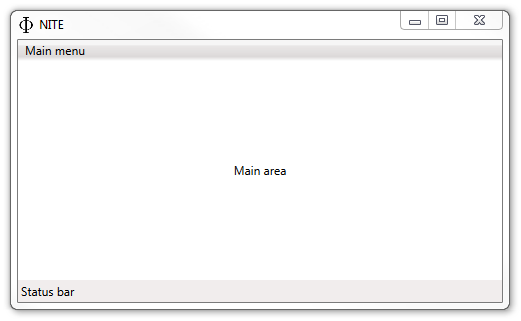
\includegraphics[width=.5\textwidth]{../../graphics/PhiniteGuiMockup.png}
  \caption{schema of the graphical user interface}
\end{figure}

\subsection{Main menu}
Main menu contains all general options that are required to be implemented, but are not connected
with a specific step of calculation. Contents of the menu must not change during application
operation, but its certain entries may be temporarily disabled during some phases of computation.

Main menu will contain, ex. exit option, %load option, 
example selection option.

\subsection{Main area}
Main area will contain frequently changing content, as it may have any of the following: a text
field for entering a regular expression, button to proceed to the next step of computation, button
to abort computation, button to display final result, a table with intermediate results, a final
result, etc. Content of main area depends on context, i.e. previous actions of the user and current
status of application.

\subsection{Status bar}
Status bar must contain one of three phrases at all times, unless there are equivalent indicators
implemented (mentioned in each point):
\begin{itemize}

  \item ``busy'' - if program computes the final or intermediate result. %, or is loading data.
  
  Equivalent of this is locking all elements of the GUI while the program is busy.

  \item ``awaiting user interaction'' - if program is not busy, but intends to be right after user
  gives some information that may help with further computation. The phrase may be changed to other
  with the same meaning. This status is intended only for computation phase, and only for those
  parts of computation phase that require user input.
  
  Equivalent of this status is displaying a new window. All information and input fields needed by
  the user to help the program must be in this new window. When it is closed, program resumes
  computation.
  
  Since the user feedback mechanism is optional (provided that it is of course substituted with
  working implementation), in certain implementation scenarios this status will never occur (or
  window will never be shown). If development team is able to prove that this feature would really
  never be used, this status indication does not have to be implemented.

  \item ``ready'' - in all other situations, for example: after start-up, %after loading the data,
  after completing the computation.
  
  Equivalent of this status is a situation in which both previous mechanisms are implemented using
  second variant. If it is so, this status can be omitted.

\end{itemize}

Status bar may also temporarily contain some optional content that may help the user in completing
the user interaction phase, provided that the main area is not a proper place for this content.

\section{Classes}
This section goes through the most important classes used in the project.

\subsection{Regular expression}
Numerous classes are required to store regular expression from its raw form up to completely parsed
form.

\begin{enumerate}

  \item First of all, \verb|PartialExpressionRole|, enumeration of roles that a given part of the
  expression can assume.

  \item \verb|UnaryOperator|, enumeration of unary operators that a given part of the expression can
  be affected by.

  \item \verb|PartialExpression|, a single node of a parse tree that stores the actual
  expression as a generative grammar.

  \item Enumeration of tags used to tag the input character sequence named \verb|InputSymbolTag|.

  \item Finally, \verb|RegularExpression|, an object that stores all the data about the regular expression.

\end{enumerate}

% \begin{minted}[mathescape,linenos,numbersep=5pt,gobble=1,tabsize=3,framesep=2mm]{csharp}
% 	public class RegularExpression
% 	{
% 		public static readonly KeyValuePair<string, InputSymbolTag>[] ReservedSymbols;
% 
% 		public static readonly Dictionary<InputSymbolTag, string> TagsStrings;
% 	}
% \end{minted}

% \begin{minted}[mathescape,linenos,numbersep=5pt,gobble=1,tabsize=3,framesep=2mm]{csharp}
% 	public enum PartialExpressionRole
% 	{
% 		EmptyWord, Letter, Concatenation, Union, Undetermined
% 	}
% \end{minted}

\begin{figure}[ht!]
  \centering
  \begin{tikzpicture}

    \begin{class}[text width=8cm]{PartialExpression}{0,0}
      %\attribute{+ Role : PartialExpressionRole}
      \attribute{+ Root : PartialExpression}
      \attribute{+ Parts : ReadOnlyCollection<PartialExpression>}
      \attribute{+ Value : string}
      %\attribute{+ Operator : UnaryOperator}
  
      \operation{+ Optimize() : void}
      \operation{+ Derive(removedLetter : string) : void}
      \operation{+ GeneratesEmptyWord() : bool}
    \end{class}

    \begin{enumeration}[text width=4cm]{PartialExpressionRole}{10,2}
      \attribute{EmptyWord}
      \attribute{Letter}
      \attribute{Concatenation}
      \attribute{Union}
      \attribute{Undetermined}
    \end{enumeration}

    \begin{enumeration}[text width=3cm]{UnaryOperator}{12,-2}
      \attribute{None}
      \attribute{KleeneStar}
      \attribute{KleenePlus}
    \end{enumeration}

    \aggregation{PartialExpressionRole}{+ Role}{1}{PartialExpression}

    \aggregation{UnaryOperator}{+ UnaryOperator}{1}{PartialExpression}

    \begin{class}[text width=11cm]{RegularExpression}{2,-7}
      \attribute{- taggedInput : List<KeyValuePair<string, InputSymbolTag> >}
      \attribute{- tagCount : Dictionary<InputSymbolTag, uint>}
      \attribute{+ Alphabet : ReadOnlyCollection<string>}
      \attribute{+ Input : string}

      \operation{+ EvaluateInput() : void}
      \operation{- TagInput() : void}
      \operation{- CountTags() : void}
      \operation{- ParseInput() : void}
      \operation{+ Optimize() : void}
      \operation{+ Derive(removedLetter : string) : RegularExpression}
      \operation{+ GeneratesEmptyWord() : bool}
    \end{class}

    \composition{PartialExpression}{- parsedInput}{1}{RegularExpression}

    \begin{enumeration}[text width=4cm]{InputSymbolTag}{11,-5}
      \attribute{Letter}
      \attribute{Union}
      \attribute{KleeneStar}
      \attribute{KleenePlus}
      \attribute{OpeningParenthesis}
      \attribute{ClosingParenthesis}
      \attribute{EmptyWord}
    \end{enumeration}

    \aggregation{InputSymbolTag}{}{1..*}{RegularExpression}

  \end{tikzpicture}
  \caption{diagram of classes related to regular expression parsing}
\end{figure}

\newpage

\subsection{Finite-state machine}
Few classes are required to store information about the constructed finite-state machine, because
most of the computational complexity is on the side of \verb|PartialExpression| class.

\begin{enumerate}

  \item \verb|MachineTransition|, that stores information about a single transition from a certain
  state to another.

  \item Finally, \verb|FiniteStateMachine|, a place to store all information about a single
  finite-state machine.

\end{enumerate}

\begin{figure}[ht!]
  \centering
  \begin{tikzpicture}

    \begin{class}[text width=13cm]{FiniteStateMachine}{0,0}
      \attribute{+ Input : RegularExpression}
      \attribute{+ InitialState : RegularExpression}
      \attribute{- notLabeled : List<RegularExpression>}
      \attribute{- notDerivedIds : List<int>}
      \attribute{- equivalentStatesGroups : List<KeyValuePair<int, List<RegularExpression> > >}
      \attribute{- notOptimizedTransitions : List<Tuple<int, string, RegularExpression> >}
      \attribute{+ States : ReadOnlyCollection<RegularExpression>}
      \attribute{+ FinalStates : ReadOnlyCollection<RegularExpression>}

      \operation{+ Construct(numberOfSteps : int) : void}
      \operation{- InitializeEvaluation() : void}
      \operation{+ LabelNextExpression() : bool}
      \operation{+ DeriveNextExpression() : bool}
      \operation{+ IsConstructionFinished() : bool}
    \end{class}
    
    \begin{class}[text width=4cm]{Tuple}{-1,6}
      \attribute{+ Item1 : int}
      \attribute{+ Item2 : List<string>}
      \attribute{+ Item3 : int}
    \end{class}

    \begin{class}[text width=5cm]{MachineTransition}{7,6}
      \inherit{Tuple}
 
      \operation{+ AddLetter(letter : string) : void}
      \operation{+ AddAllLetters(letters : IEnumerable<string>) : void}
    \end{class}

    \composition{MachineTransition}{+ Transitions}{0..*}{FiniteStateMachine}
    %\unidirectionalAssociation{RegularExpression}{Input}{1}{FiniteStateMachine}

  \end{tikzpicture}
  \caption{diagram of classes needed for finite-state machine related tasks}
\end{figure}

The development team must preserve the types and names of all public properties of all types
mentioned in the two above sections. The names and return types of pulbic methods also have to be
preserved. The names of all listed classes and enumerations also have to be exactly as specified.
All public properties must be treated as read-only - some backing fields should be created and used
for processing.

Other names and types can be changed, added or removed at will, provided that this is a properly
justified decision, and all of the names still carry a meaning corresponding to their true role. The
development team may also add some other classes that are used internally during the processing. One
exception: the \verb|parsedInput| field cannot be removed or changed.

\newpage

\section{Algorithms}

\subsection{Conversion of plain text into a RegularExpression object}
The algorithm should follow the standard procedure applied in the are of natural language
processing. Of course in case of this algorithm that process is simplified greatly because of the
fact that we do not parse a human language but a machine language.

\subsubsection{Tagging}
First step is to tag the input data accordingly. This is done for several reasons:

\begin{enumerate}

  \item As the tagging is done, algorithm eliminates ignored symbols by not adding them to the
  tagged input.

  \item The tagging eliminates the difference between letters, all non-special symbols are simply
  regarded as ``letters''. From the point of view of further parsing, this greatly simplifies the
  process.

  \item As the input is tagged, it becomes much easier to detect which parts of it belong together.

  \item The validation and therefore stopping in case of some mistakes like open bracket without a
  corresponding closing one, or placing a unary operator after an opening bracket, etc. is
  simplified.

\end{enumerate}

Program shall go through all the letters and assign a tag to each of them. The direction of the
processing (left to right or right to left) does not matter. In fact, the solution can, but does not
have to be, parallelized. In case of sequential solution the worst case running time must be $O(n)$,
in case of parallel solution $O(n/k)$ assuming $k$ is the number of cores used, $k \leq n$.

The developer should pay attention to the fact that some special symbols consist of several
characters. In such cases a single tag is placed over all of the characters that constitute such
symbol. Therefore the parallelization may add some complications.

Results of tagging are stored in \verb|taggedInput| field. Relevant tag counts in the
\verb|tagCount| field are incremented on-the-go.

\subsubsection{Tag counting}
In this step the algorithm simply checks (using already prepared \verb|tagCount| field) the counts
of parentheses to ensure that there is the same number of opening and closing ones.

\subsubsection{Parsing}
Third step is to parse the tagged input into a tree. A tree created by parsing a plain text using a
certain grammar is called a parse tree in research texts related to natural language processing.

The steps of the algorithm and definitions used later on:
\begin{enumerate}

  \item a new, empty \verb|PartialExpression| is created and it becomes a current part

  \item current part is always labeled as ``Part''

  \item Part becomes a root part of the currently created parse tree

  \item root of the current parse tree is always labeled as ``Root''

  \item the role of Part is set to \verb|Undetermined|

  \item role of the current part is always labeled as ``Role''

  \item the algorithm goes through all characters of the input, starting from the first

  \item at each step, the currently evaluated symbol is labeled as ``Symbol''

  \item at each step, the actions of the algorithm depend on the Role, Symbol and Root; these
  actions are described in a separate table that follows

  \item if there are no more symbols to parse, the part that is Root is set as a root of the parse
  tree of the whole regular expression (field \verb|parsedInput| of \verb|RegularExpression|)

\end{enumerate}

The procedure is a recursive one. Parentheses are the triggers for recursion. The below table shows
the behaviour of the algorithm. This table is a human-readable version of an underlying grammar that
is used to create the parse tree.

\vspace{10pt} \noindent
\begin{tabularx}{\textwidth}{l|l|l|X}

Role & Symbol & Root & result \\ \hline

\verb|Undetermined| & \verb|EmptyWord| & $*$ &

1) Role is set to \verb|Concatenation| \newline
2) a new part with role \verb|EmptyWord| is added to parts of Part \\

\verb|Undetermined| & \verb|Letter| & $*$ &

1) Role is set to \verb|Concatenation| \newline
2) and a new part with role \verb|Letter| and value of the Symbol is added to parts of Part \\

\verb|Concatenation| & \verb|EmptyWord| & $*$ &

a new part with role \verb|EmptyWord| is added \\

\verb|Concatenation| & \verb|Letter| & $*$ &

a new part with role \verb|Letter| and value of the Symbol is added \\

\verb|Concatenation| & \verb|Union| & $\equiv$Part &

1) a new part with role \verb|Union| is created, and this new part is set as Root; \newline
2) Part is added to the list of parts of Root (becoming the first part in this list) \newline
3) a new part with \verb|Undetermined| role is created, it is appended to the parts of the Root and
it is set as Part \\

\verb|Concatenation| & \verb|Union| & $\not\equiv$Part &

%1) a new part with role \verb|Union| is created, and this new part is set as Root; \newline
%1) Part is added to the parts of Root \newline
a new part with \verb|Undetermined| role is created, it is appended to the parts of the Root and
it is set as Part \\

\verb|Concatenation| & \verb|OpeningParenthesis| & $*$ &

1) the sub-procedure of parsing starts from step one (see algorithm), and the sub-procedure treats the first
symbol after the parenthesis as the first symbol of input \newline
2) when the sub-procedure ends, the returned partial expression is appended to the list of parts of Part \newline
3) the procedure skips all symbols parsed by the sub-procedure and continues \\

\verb|Concatenation| & \verb|ClosingParenthesis| & $*$ &

the parsing sub-procedure ends, Root is returned \\

\verb|Concatenation| & \verb|KleeneStar| & $*$ &

the operator of the last of the parts of Part is set to \verb|KleeneStar| \\

\verb|Concatenation| & \verb|KleenePlus| & $*$ &

the operator of the last of the parts of Part is set to \verb|KleenePlus| \\

\end{tabularx}

\vspace{10pt} All other encountered pairs of Role-Symbol result in an undefined behaviour. Such pairs would
however violate the rules of the underlying grammar, therefore they can, and shall be detected in
the tagging step. Also, in the table there are some assumptions about data integrity which are
ommited. Catching of invalid tag sequences in before starting parsing phase and correct
implementation of the above algorithm ensures data integrity i.e. ensures that the correct parse
tree will be built.

\subsubsection{Optimization}
The fourth and the last phase is to optimize the parse tree i.e. eliminate any redundant productions
and useless symbols. This step is optional, but highly recommended.

Parse tree has redundant productions if its underlying grammar can generate the same word using more
than one set of productions. Eliminating the redundant productions means that the grammar still
generates the same language, but fewer (or no) productions are redundant.

Below is the list of patterns that are considered not optimal, together with methods of optimization:
\begin{enumerate}

  \item A part that has role of \verb|Concatenation| or \verb|Union|, and has only one part - it
  shall be converted to the part itself.

  In this case special rules regarding operators apply:

  \noindent
  \begin{tabular}{c|c|c}
  Operator of parent & Operator of its single part & resulting operator \\ \hline
  \verb|None| & $*$ & $*$ \\
  $*$ & \verb|None| & $*$ \\
  \verb|KleeneStar| & $*$ & \verb|KleeneStar| \\
  $*$ & \verb|KleeneStar| & \verb|KleeneStar| \\
  \verb|KleenePlus| & \verb|KleenePlus| & \verb|KleenePlus| \\
  \end{tabular}

  \vspace{10pt} The algorithm shall analyze if the rules apply to the current situation from top to
  bottom, and apply the first matching rule.

  \item A part that is a part of \verb|Concatenation| and its role is equal to \verb|EmptyWord| -
  such part can be deleted altogether unless it is the only part of that \verb|Concatenation|.

  \item If a \verb|Union| has some parts that are equal, the duplicates can be safely deleted.

  \item If we have two consequtive parts of a \verb|Concatenation| that satisfy all of the following conditions:

  \begin{itemize}

    \item both have unary operators

    \item those unary operators may be different or the same

    \item without taking operators into account, these parts are equal

  \end{itemize}

  then, one of the parts can be safely removed provided that the operator of the other part is
  modified accordingly:

  \noindent
  \begin{tabular}{c|c|c}
  initial operator & operator & resulting operator \\
  of the remaining part & of removed part & of the remaining part \\ \hline
  \verb|KleeneStar| & \verb|KleeneStar| & \verb|KleeneStar| \\
  \verb|KleeneStar| & \verb|KleenePlus| & \verb|KleenePlus| \\
  \verb|KleenePlus| & \verb|KleenePlus| & \verb|KleenePlus| \\
  \verb|KleenePlus| & \verb|KleeneStar| & \verb|KleenePlus| \\
  \end{tabular}
  
  %\vspace{10pt}
  %and cases where operators are identical are covered by point 2. of this list.

  \item If we have a pair of parts of a \verb|Union|, which are placed anywhere in the union, that
  satisfy all of the following conditions:

  \begin{itemize}

    \item either both of them have any (but different) unary operator, or one of them has
    \verb|KleenePlus| and the other has no operator

    \item without taking operators into account, these parts are equal

  \end{itemize}

  then, one of the parts can be safely removed provided that the operator of the other part is
  modified accordingly:

  \noindent
  \begin{tabular}{c|c|c}
  initial operator & operator & resulting operator \\
  of the remaining part & of removed part & of the remaining part \\ \hline
  \verb|KleenePlus| & \verb|None| & \verb|KleenePlus| \\
  \verb|None| & \verb|KleenePlus| & \verb|KleenePlus| \\
  \verb|KleeneStar| & \verb|KleenePlus| & \verb|KleeneStar| \\
  \verb|KleenePlus| & \verb|KleeneStar| & \verb|KleeneStar| \\
  \end{tabular}
  
  \vspace{10pt}
  and cases where operators are identical are covered by point 3. of this list.

  \item If some part $x$ is a is a \verb|Concatenation|, it has no operator, and it is a part of
  another \verb|Concatenation| $y$, which also has no operator, then all parts of $x$ can be moved
  into $y$.

  For example: $y = ay$, $x = bc$, then, instead of having $y = a(bc)$, we can safely have $y = abc$

  \item If some part $x$ is a is a \verb|Union|, it has no operator, and it is a part of another
  \verb|Union| $y$, which also has no operator, then all parts of $x$ can be moved into $y$.

  For example: $y = a+y$, $x = b+c$, then, instead of having $y = a+(b+c)$, we can safely have $y =
  a+b+c$

  \item If some partial expression is a \verb|Union| and has \verb|KleeneStar|, then every its part
  that is a \verb|EmptyWord| can be safely deleted, beceause the empty word will be generated
  anyway.

  For instance: $(a+\epsilon+b)^* \equiv (a+b)^*$

\end{enumerate}

This step is needed to ensure that the implementation second algorithm can be greatly simplified.
The implementation of the second algorithm becomes much more difficult without assumption that the
parse tree is optimal.

It is still possible to implement the derivation and labeling algorithm without optimizations, that
is why the implementation of optimization is not mandatory.

\newpage

\subsection{Conversion of RegularExpression object into FiniteStateMachine object}

\writehere

\subsubsection{Initialization}

\writehere

\subsubsection{Step-by-step construction}

The two following (labeling and derivation) steps are executed in the loop, until the computation is
complete. Conditions for ending the computation are described in relevant section later on.

Splitting the computation into loop consisting of small, repetative steps, is necessary for
implementation of step-by-step computation. When immediate result is needed, a loop can be simply
set to run without interruption.

\subsubsection*{Labeling step}

\begin{enumerate}

  \item The first element from \verb|notLabeled| list is taken, it becomes the current element:
  ``Element''.

  \item If \verb|equivalentStatesGroups| is empty:

  \begin{itemize}
    \item the Element is added to that list with $key = 0$
  \end{itemize}

  else:

  \begin{enumerate}

    \item The \verb|equivalentStatesGroups| list is checked whether it contains Element. If it does,
    the algorithm goes to point 3.

    \item if it does not, then the algorithm breaks and the user is prompted to provide his opinion
    regarding the Element, i.e. if in user's opinion some state from \verb|States| is equivalent to
    the Element.

    \item When the user answers false, the algorithm continues and adds new entry to
    \verb|equivalentStatesGroups|, with new $key = $\verb|equivalentStatesGroups.Count| and goes to point 3.

    \item When the users indicates to what already labeled state the Element is equivalent, the
    algorithms adds a new state to the list of states with $key$ equal to the user indicated state
    number - in the field \verb|equivalentStatesGroups|.

  \end{enumerate}

  \item Algorithm iterates through \verb|notOptimizedTransitions| and for each its entry that has
  the resulting state equal to Element.

  \begin{enumerate}

    \item Adds a new \verb|MachineTransition| to \verb|Transitions| with the corresponding ids and
    letter(s).

    \item Removes the entry from \verb|notOptimizedTransitions|.

  \end{enumerate}

  \item The Element is removed from \verb|notLabeled| list.

\end{enumerate}

\subsubsection*{Derivation step}

\begin{enumerate}

  \item The first element from \verb|notDerivedIds| list is taken, then its corresponding element from
  \verb|equivalentStatesGroups| is taken and it becomes the derived element: ``Element''.

  \item The Element is derived for each letter that exist in its alphabet. The derivation procedure
  is as follows:
  
  \begin{enumerate}

    \item A copy of parse tree of Element is made, this copy becomes the currently processed tree.

    \item Currently processed tree is alwayes labeled ``Tree''.

    \item The Tree is processed using the rules contained in the tables that follow. In that tables:
    Role is simply the role of Tree, Operator is the Tree's unary operator.
    
    \item At first the transformations from the first table are applied, then those from the second.

    \item A new \verb|RegularExpression| object is created from a transformed Tree, and it
    becomes the derived element.

  \end{enumerate}

  \item for each derived element:

  \begin{itemize}

    \item if derivation is not null (that is equivalent to entering the rejecting state), a new
    entry is added to a list of not optimized transactions: \verb|notOptimizedTransitions|, and that
    entry has: a) the id from \verb|notDerivedIds| corresponding to Element (exactly the same as in
    step 1.), b) the letter by which the derivation was made, and of course c) the result of
    derivation

  \end{itemize}

  \item the id of Element is removed from \verb|notDerivedIds|

\end{enumerate}

The first table with transformations:

\vspace{10pt}
\noindent
\begin{tabularx}{\textwidth}{l|X}

Operator & actions \\ \hline

\verb|None| & none \\ \hline

\verb|KleeneStar| &

1) new part with copy of Tree is created, but copy's operator is set to \verb|None|; \newline
2) new part with copy of Tree is created; \newline
3) a \verb|Concatenation| of parts from 1) and 2) is created; \newline
4) new part that is an \verb|EmptyWord| is created; \newline
5) Role is set to \verb|Union|; \newline
6) Operator is set to \verb|None|; \newline
7) All Tree parts are removed; \newline
8) part from 4) is added to Tree parts; \newline
9) part from 3) is appended to Tree parts \\ \hline

\verb|KleenePlus| &

1) new part with copy of Tree is created, but copy's operator is set to \verb|None|; \newline
2) new part with copy of Tree is created, but copy's operator is set to \verb|KleeneStar|; \newline
%3) a \verb|Concatenation| of parts from 1) and 2) is created; \newline
%4) new part that is an \verb|EmptyWord| is created; \newline
3) Role is set to \verb|Concatenation|; \newline
4) Operator is set to \verb|None|; \newline
5) All Tree parts are removed; \newline
6) part from 1) is added to Tree parts; \newline
7) part from 2) is appended to Tree parts \\

\end{tabularx}

\vspace{10pt}
The second table with transformations:

\vspace{10pt}
\noindent
\begin{tabularx}{\textwidth}{l|X}

Role & actions \\ \hline

\verb|EmptyWord| &

Role is set to \verb|Invalid| \\ \hline

\verb|Letter| &

if value equals to that of derived letter, Role is set to \verb|EmptyWord|, otherwise Role is set to
\verb|Invalid| \\ \hline

\verb|Concatenation| &

\textbf{if} 1st part is a union that has empty word:

?

\vspace{5pt}
\textbf{else if} 1st part has a \verb|KleeneStar| operator:

?

\vspace{5pt}
\textbf{else}:

for the first part of Tree, launch the derivation sub-procedure where only steps from 2.(b) to 2.(d)
are executed \\ \hline

\verb|Union| &

for each part in Tree parts, launch a derivation sub-procedure where only steps from 2.(b) to 2.(d)
are executed \\

\end{tabularx}

\subsubsection{Ending the computation}

Computation is regarded as complete when after the derivation step, both \verb|notLabeled| and
\verb|notDerived| lists are empty.

\subsection{Evaluation of a given word using FiniteStateMachine object}

\writehere

\end{document}
